\documentclass[12pt]{article}
\title{Part IIA Paper 3 Project}
\author{
	Anonymous
}

\newcommand\wordcount{
	\immediate\write18{texcount -sum -1 \jobname.tex > count.txt} 
	\input{count.txt}
}

\usepackage[a4paper, total={6.25in, 10in}]{geometry} % to adjust the margins etc
\usepackage{titlesec} % for the title formatting
\usepackage{setspace} % to set line spacing
\usepackage[parfill]{parskip} % remove the paragraph indentation
\usepackage{caption} % used to allow smaller "notes" under graphs/tables besides the main caption
\usepackage{booktabs} % used for the lines under the headers in the tables
\usepackage{multirow} % to allow multiple row option in table formatting
\usepackage{array} % for struts in formatting table
\usepackage{fancyhdr} % for moving page number to the bottom right corner
\usepackage{amsmath} % for multi line equations aligning
\usepackage{bm} % for bolded math symbols (for vectors)
\usepackage{graphicx}

\titleformat*{\section}{\centering \LARGE}
\pagenumbering{arabic} % add page numbers
% next few lines are to get the page numbers to the bottom right
\pagestyle{fancy}
\fancyhf{}
\renewcommand{\headrulewidth}{0pt}
\fancyfoot[R]{\thepage}


\begin{document}
	\maketitle
	\begin{spacing}{1.5} % set 1.5 line spacing
		Q1. Vaccination take-up rates: Inter-State differences in the USA in 2021.
		
		At the end of 2021 the share of the population fully vaccinated against Covid-19 differed widely across US States.
		
		a) Identify and evaluate the main economic and social factors giving rise to this outcome.
		
		b) On the basis of your answer to a), suggest how high vaccination rates might be achieved across the entire United States.
		
		\wordcount words
		\section{Introduction}
		Hello world hi hi hello d
		
		By the end of 2021, only 2\% of people wanted a vaccine and had not yet got it, from survey
		
		\section{Data and Methods}
		\subsection{Data}
		Regressions were generally done on the county level. Data on vaccination rates across time by county (and by state) were all sourced from the CDC (CITE). A dataset of time-invariant characteristics of each county was also compiled from many sources for 3075 counties in the United States; remaining counties were excluded due to some or all information not being available for them. This includes all US territories (such as Puerto Rico), which do not have presidential voting records, and all counties in Alaska and Hawaii. Utah's counties were also excluded due to spotty COVID-19 case data. Outside of these states, the following counties also had missing records: Bedford and Clifton Forge City, Dukes, Nantucket, Barnstable, and Ogala Lakota County, and Yellowstone National Park (which has no population).
		
		2020 election results by county were obtained from the MIT Election Data and Science Lab's Election Returns Dataverse (CITE). Religious breakdowns by county were obtained from the Public Religion Research Institute (PRRI) 2020 census of American Religion (CITE). Education attainment by county, averaged over 2015-2019, was obtained from the US Census Bureau ('the Census'), via the 2015-2019 American Community Survey (CITE). Poverty rates by county in 2019 were obtained from the Census' Small Area Income and Poverty Estimates, which also contained the 2013 Rural-Urban Continuum Code assigned to each county, which classifies counties based on their level of urbanization and proximity to metropolitan areas (CITE explanation). Racial breakdowns by county were obtained from the 2020 Decennial Redestricting Dataset, maintained by the Census (CITE). Age breakdowns by county were obtained from the County Characteristics Resident Population Estimates maintained by the Census (CITE). Median family incomes and costs of living for a family of four were obtained from the Economic Policy Institute's (EPI) Family Budget Calculatior (CITE).  COVID-19 Cases recorded in each county, as of 1 December 2020, were obtained from the CSSE COVID-19 Data Repository maintained by John Hopkins (CITE). Finally, data mapping each county to every county it borders was obtained (the 'county adjacency dataset') from a dataset maintained by the National Bureau of Economic Research (CITE), originating from a dataset maintained by the Census. 
		
		All datasets tagged each county with their Federal Information Processing Standard Publication (FIPS) codes, which was used to merge them together.
		% commentary on different years for data
		\subsection{Methods}
		As mentioned, vaccine access seems to not have been a substantial problem by the end of 2021. Instead, vaccination status reflects the willingness of individuals to get vaccinated.
		
		The decision on vaccination can reasonably be broken down into its costs and benefits, and beliefs that agents have about them. We would expect, hence that in areas of lower population density, or where COVID would generally spread less quickly, the benefit of vaccination would be lower. Furthermore, as COVID-19 has a much higher fatality rate among older persons (CITE), they would find a greater benefit to vaccination, and we would expect more vaccination, in counties with more elderly people. As beliefs on vaccination's benefits and supposed harms seem to be affected by, or at least correlated with, religious status, race, and political identity, we also expect these variables.
		
		We begin hence by first running the following cross-sectional regression on the national dataset of 3075 counties:
		
		\begin{equation} \label{eq:crosssection}
			\begin{split}
				\textrm{vaccuptake}_i = &\beta_0 + \beta_1 \textrm{repvotes}_i + \beta_2 \textrm{whiteevangelical}_i + \beta_3 \textrm{catholic}_i \\ 
				&+ \beta_4 \textrm{black}_i + \beta_5 \textrm{poverty}_i + \beta_6 ln(\textrm{medincome}_i) + \beta_7 ln(\textrm{col}_i) \\ 
				&+ \beta_8 \textrm{pop60to79}_i + \beta_9 \textrm{above80}_i + \beta_{10} \textrm{fullcollege}_i + \beta_{11} \textrm{casespc}_i \\
				&+\boldsymbol{\delta}\cdot \mathbf{rural}_i + \boldsymbol{\gamma}\cdot \mathbf{state}_i + u_i
			\end{split}
		\end{equation}
		
		Where $\textrm{vaccuptake}_i$ is a measure of vaccine uptake for a county $i$. Definitions for each covariate are listed in Table \ref{table:definition}. The model was estimated for a cross-section of vaccine uptake by county as of 31 December 2021, and also for vaccine uptake as of 1 June 2021, to see if the effects of the covariates on uptake had changed over time. We measured vaccine uptake as the percentage of county residents who had taken at least two doses of the vaccine, and also an alternatively looked at the percentage of county residents who had taken at least one dose of the vaccine, in case effects were substantially different between the two.
		
		\begin{table}
			\caption{Variable Definitions}
			\begin{minipage}{6.5in}
	\centering
	\def\sym#1{\ifmmode^{#1}\else\(^{#1}\)\fi}
	\def\arraystretch{1}
	\begin{tabular*}{\textwidth}{@{\extracolsep{\fill}}lp{0.35\linewidth}p{0.4\linewidth}}
	\hline\hline
		&Definition&Justification\\
		\hline
		repvotes&Percentage (0-100) of county vote that Donald Trump received in the 2020 election&Aim to measure effect of political affiliation, which affects news consumption and beliefs on the costs and benefits of vaccination\\
		whiteevangelical&Percentage (0-100) of county identifying as White Evangelical Protestants as of 2020&Aim to measure effect of religion - White Evangelicals are a heavily conservative and Republican-supporting religious group. (CITE)\\
		catholic&Percentage (0-100) of county identifying as Catholics as of 202&Aim to measure the effect of religion - the Pope has actively extolled the benefits of vaccination (CITE), check effect.\\
		black&Percentage (0-100) of county who are African-American as of 2020&Due to historical grievances and mistrust of government, African-Americans are known to be less likely to choose to vaccinate. (CITE)\\
		poverty&Percentage (0-100) of county under the poverty line as of 2019(as defined by the Census)&Those in poverty may have difficulty finding access to vaccines, or more broadly, access to good-quality information on their costs and benefits.\\
		medincome&Nominal median family income for a family of four, as of 2020&Same reason as above. Poverty variable lets us see if effect is stronger at the low end of the income distribution.\\
		col&Cost of living as of 2020, as measured by the EPI.&Allows coefficient on medincome to be interpreted as the effect of changes in real median income (holding prices/cost of living fixed)\\
		pop60to79&Percentage (0-100) of county aged between 60 and 79 in 2019.&Elderly are at greater risk of death and serious illness from COVID-19\\
		above80&Percentage (0-100) of county aged 80 and above in 2019&See above\\
		fullcollege&Percentage (0-100) of county who completed at least 4 years of college, averaged 2015-2019&Those with college degrees may be less susceptible to misinformation on the supposed harms of vaccination\\
		casespc&Total recorded COVID-19 cases as of 1 December 2020, before the start of the vaccination program.&A proxy for how amenable the area is to COVID-19 spread, which would increase the benefit of vaccination against COVID-19\\
		$\mathbf{rural}$&Vector of dummy variables for each possible score on the 2013 Rural-Urban Continuum Code&More rural areas typically have lower population density and hence less risk of catching COVID-19, and so there are lower benefits to vaccination.\\
		$\mathbf{state}$&Vector of state fixed effects&Allows for variation in state policy responses that affected COVID-19 vaccination rates\\
	\hline\hline
	\end{tabular*}
\end{minipage}

			\label{table:definition}
		\end{table}
	
		As the various covariates having different units and standard deviations, interpreting their relative effect sizes (ie, which variables are "more important" in explaining variation in vaccine up take) can be difficult. I hence also estimated the \textit{beta coefficients} of the model - these are calculated by using the z-score of every variable (defined for a covariate $x_j$, with a sample standard deviation $\hat{\sigma}_j$, as $z_j := \frac{x_{ij}-\bar{x}_j}{\hat{\sigma}_j}$)) and noticing then that, if Model (\ref{eq:crosssection}) holds, then it is also true that
		\begin{equation} \label{eq:standardized}
			z_y=\frac{y_i-\bar{y}}{\hat{\sigma}_y} = \sum_{j=1}^{k} \frac{\hat{\sigma}_j}{\hat{\sigma}_y}\beta_j z_{ij}
		\end{equation}
		
		Hence, we can calculate, for each covariate $x_j$, a beta coefficient $\hat{b}_j := \frac{\hat{\sigma}_j}{\hat{\sigma}_y}\beta_j$, interpreted as the standard deviation change in in $y_i=\textrm{vaccuptake}_i$ (in this context) frome a one standard deviation change in covariate $x_j$. This in a sense standardizes the units across the covariates and makes them more directly comparable (although, not perfectly so, as some covariates are drawn from more-spread-out distributions).
		
		\begin{figure}
			\centering
			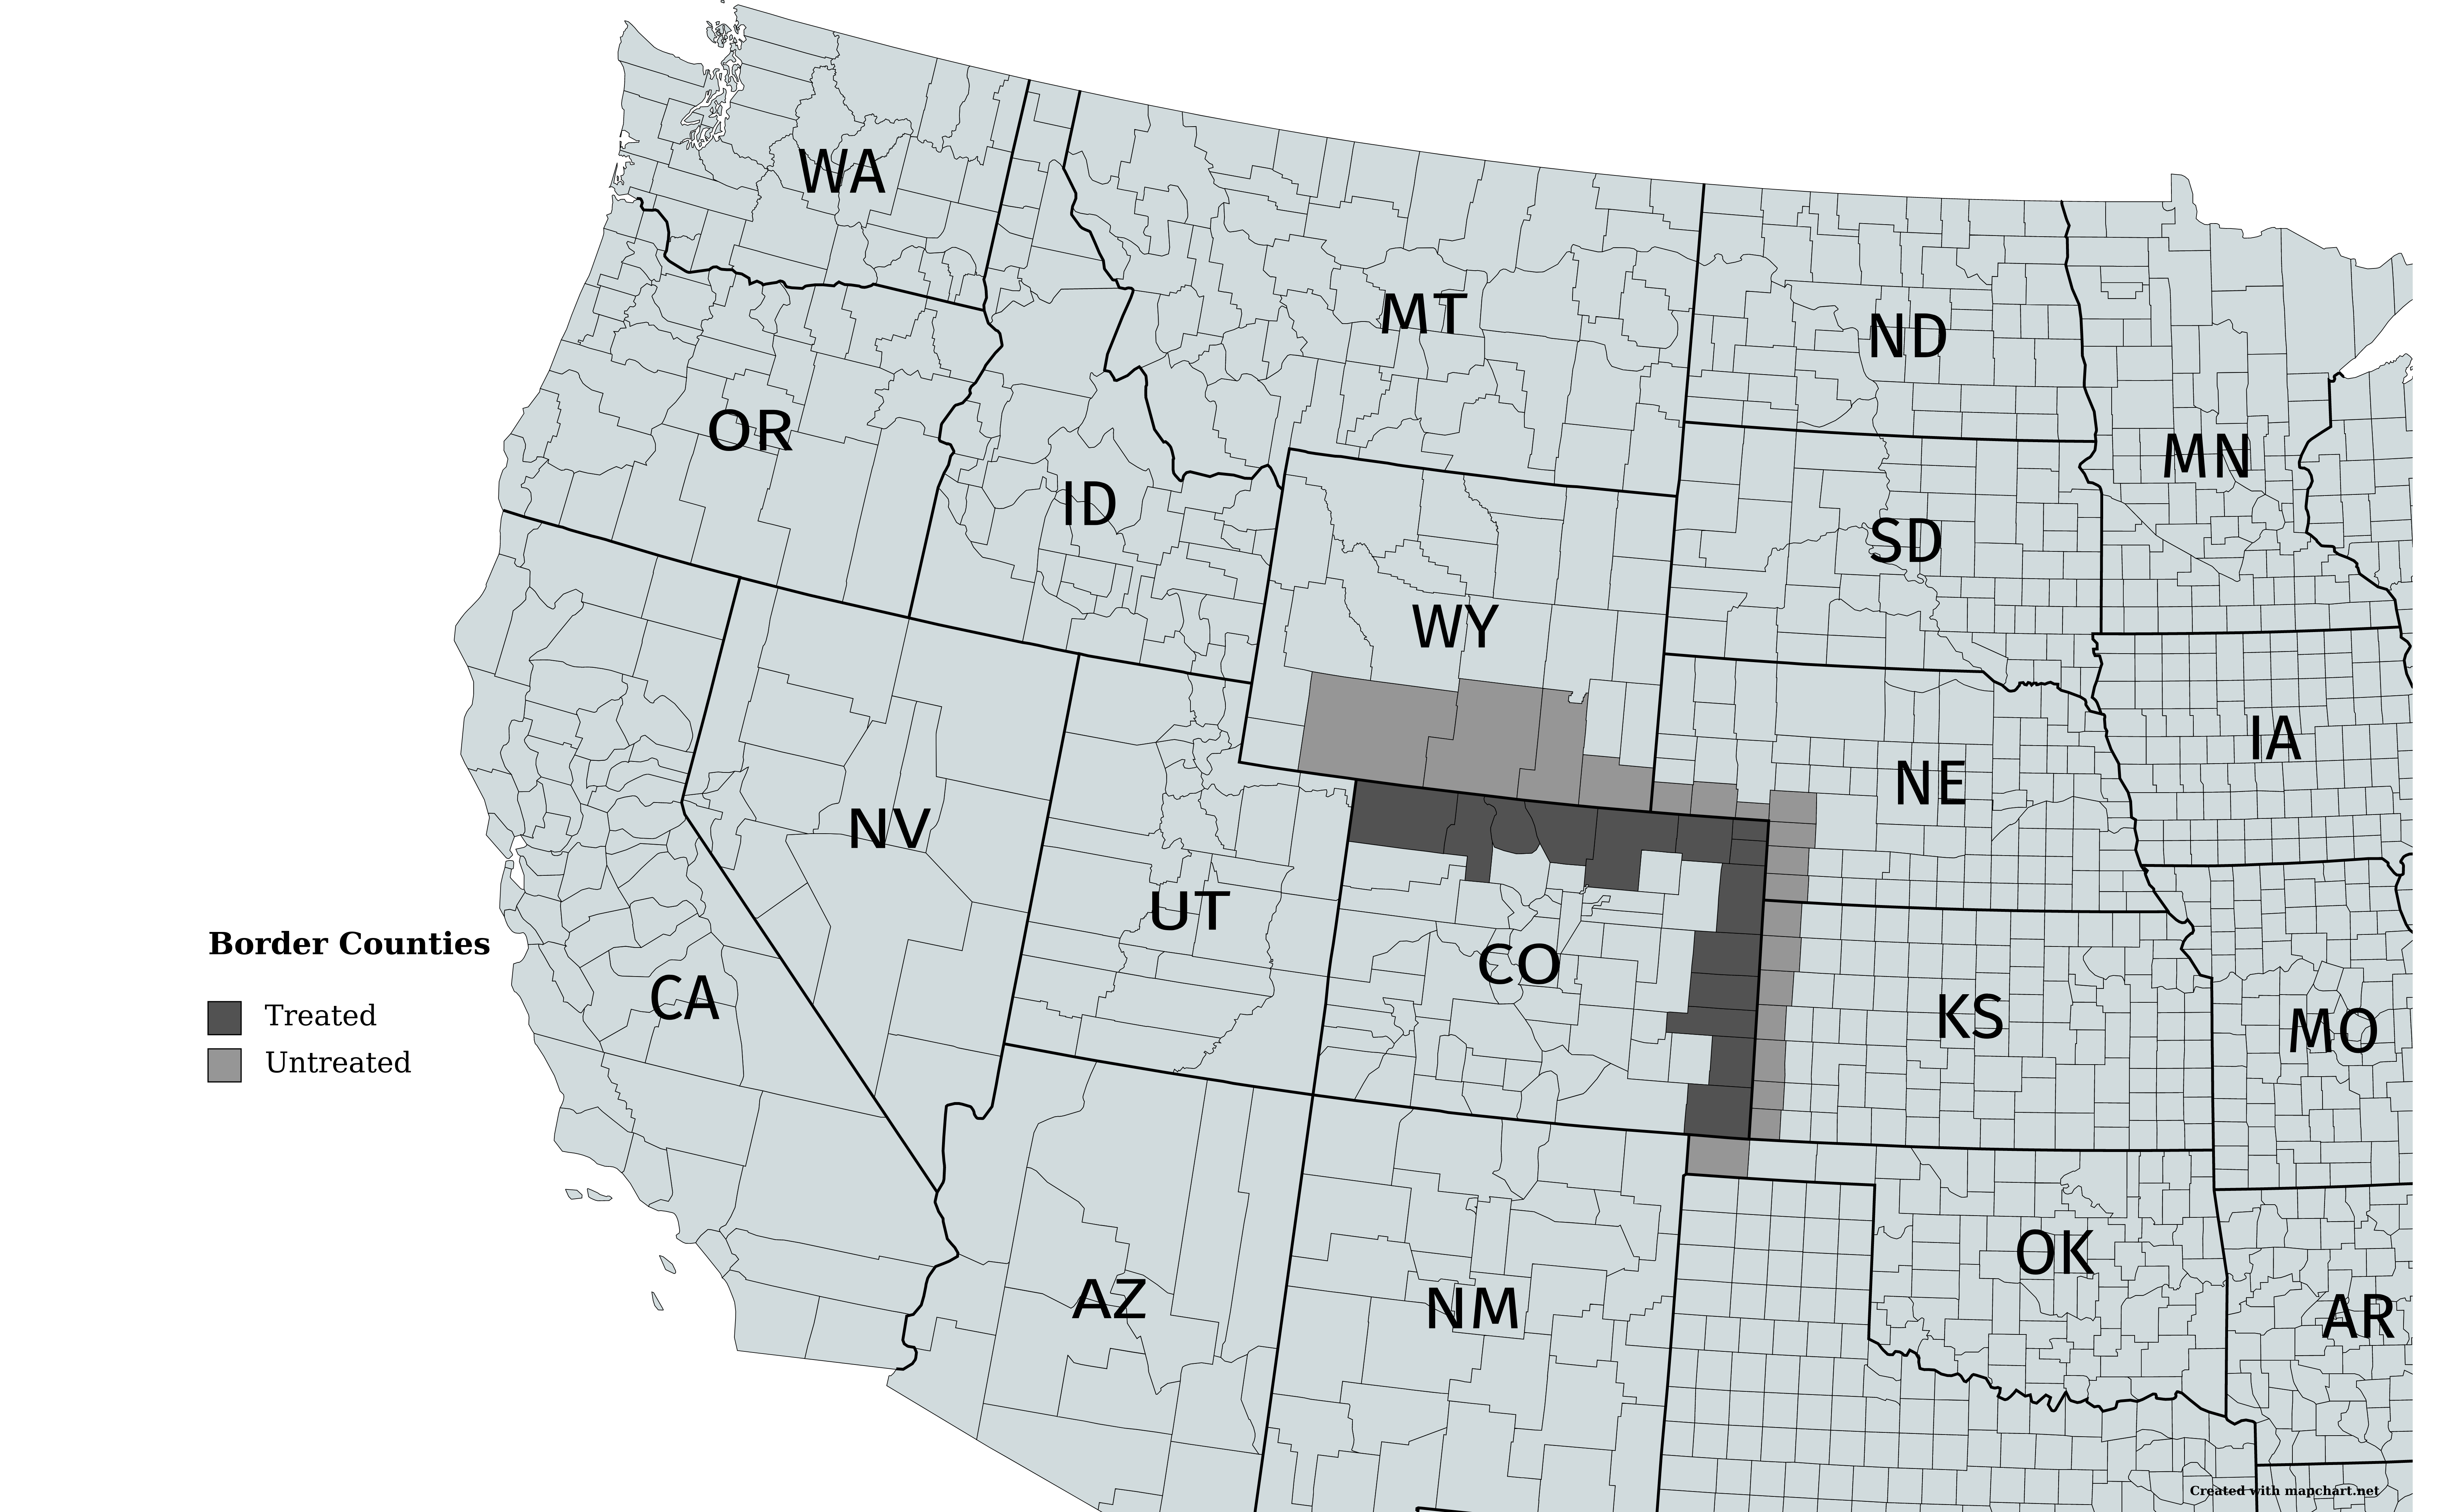
\includegraphics[width=6in]{../graphs/Border_Counties.png}
			\caption*{\footnotesize{Description of figure}}
			\caption{Counties in Pair Design}
			\label{fig:bordercounties}
		\end{figure}
		
		\begin{table}
			\centering
			\caption{Cross-Section Regression}
			\centerline{\begin{minipage}{6.5in}
	\centering
	\def\sym#1{\ifmmode^{#1}\else\(^{#1}\)\fi}
	\def\arraystretch{1.1}
	\begin{tabular*}{\textwidth}{@{\extracolsep{\fill}}l*{5}{cc}}
	\hline\hline
				&\multicolumn{3}{c}{December 31 Sample}     & \multicolumn{2}{c}{June 2 Sample}\\
				\cmidrule{2-4}\cmidrule(l{1ex}r{1ex}){5-6}
	            &\multicolumn{1}{c}{(1)}         &\multicolumn{1}{c}{(2)}&\multicolumn{1}{c}{(3)}         &\multicolumn{1}{c}{(4)}         &\multicolumn{1}{c}{(5)}\\
	            &        \multirow{2}{*}{Two Doses}        &    Two Doses    &       \multirow{2}{*}{One Dose}         &        \multirow{2}{*}{Two Doses}         &        Two Doses\\
	            &&Standardized&&&Standardized\\ 
	\hline
	\multirow{2}{*}{repvotes}&       -0.52\sym{***}&       -0.65&       -0.60\sym{***}&       -0.31\sym{***}&       -0.35\\
	            &      (0.03)         &            &      (0.04)         &      (0.03)         &            \\
	\multirow{2}{*}{whiteevangelical}&       -0.03         &       -0.03&       -0.05         &       -0.04         &       -0.03\\
	            &      (0.06)         &            &      (0.07)         &      (0.05)         &            \\
	\multirow{2}{*}{catholic}    &        0.11\sym{*}  &        0.09&        0.14\sym{**} &       -0.02         &       -0.02\\
	            &      (0.04)         &            &      (0.05)         &      (0.04)         &            \\
	\multirow{2}{*}{black}       &       -0.25\sym{***}&       -0.29&       -0.27\sym{***}&       -0.16\sym{***}&       -0.17\\
	            &      (0.03)         &            &      (0.04)         &      (0.03)         &            \\
	\multirow{2}{*}{poverty}     &       -0.15         &       -0.07&       -0.14         &       -0.13\sym{*}  &       -0.05\\
	            &      (0.08)         &            &      (0.10)         &      (0.06)         &            \\
	\multirow{2}{*}{lmedincome}  &        2.22         &        0.04&        1.33         &        4.01         &        0.07\\
	            &      (2.96)         &            &      (3.46)         &      (2.28)         &            \\
	\multirow{2}{*}{lcol}        &        4.19         &        0.04&        6.37         &        0.41         &        0.00\\
	            &      (3.41)         &            &      (4.19)         &      (3.01)         &            \\
	\multirow{2}{*}{pop60to79}   &        0.18\sym{*}  &        0.06&        0.20\sym{*}  &        0.31\sym{***}&        0.10\\
	            &      (0.08)         &            &      (0.10)         &      (0.06)         &            \\
	\multirow{2}{*}{above80}     &        0.73\sym{***}&        0.08&        0.43         &        0.53\sym{**} &        0.06\\
	            &      (0.21)         &            &      (0.26)         &      (0.17)         &            \\
	\multirow{2}{*}{fullcollege} &        0.10\sym{*}  &        0.07&        0.11\sym{*}  &        0.11\sym{***}&        0.08\\
	            &      (0.04)         &            &      (0.05)         &      (0.03)         &            \\
	\multirow{2}{*}{casespc}&       57.27\sym{***}&        0.11&       55.28\sym{**} &       52.05\sym{**} &        0.09\\
	            &     (15.05)         &            &     (16.87)         &     (16.25)         &            \\
	Constant      &        2.87         &            &        4.21         &      -11.61         &            \\
	            &     (41.54)         &            &     (50.46)         &     (33.07)         &            \\
	rural Wald Statistic&0.72&&1.59&1.08&\\
	\hline
	\(N\)       &        3075         &        3075&        3075         &        3075         &        3075\\
	White Test F-Stat&1.274&&52.24\sym{***}&5.16\sym{**}&\\
	\hline\hline
	\end{tabular*}
	\caption*{\footnotesize{Notes:\\ 
	\sym{*} \(p<0.05\), \sym{**} \(p<0.01\), \sym{***} \(p<0.001\)}}
\end{minipage}
}
			\label{table:crosssection}
		\end{table}
		
		\begin{table}
			\centering
			\caption{Coefficient Change Over Time}
			\centerline{{
\def\sym#1{\ifmmode^{#1}\else\(^{#1}\)\fi}
\begin{tabular}{l*{2}{c}}
\hline\hline
            &\multicolumn{1}{c}{(1)}&\multicolumn{1}{c}{(2)}\\
            &\multicolumn{1}{c}{fullvaxpct}&\multicolumn{1}{c}{fullvaxpct}\\
\hline
c.t c.repvotes2020pct&     -0.0323\sym{***}&     -0.0489\sym{***}\\
            &   (0.00321)         &   (0.00558)         \\
[1em]
c.t c.whiteevangelical&     0.00238         &      0.0148         \\
            &   (0.00515)         &   (0.00792)         \\
[1em]
c. c.catholic&      0.0198\sym{***}&      0.0131\sym{*}  \\
            &   (0.00415)         &   (0.00651)         \\
[1em]
c.t c.black &     -0.0112\sym{***}&    -0.00437         \\
            &   (0.00266)         &   (0.00460)         \\
[1em]
c.t c.poverty&    -0.00860         &     -0.0691\sym{***}\\
            &   (0.00704)         &    (0.0118)         \\
[1em]
c.t c.lmedincome&      -0.223         &      -1.213\sym{**} \\
            &     (0.277)         &     (0.401)         \\
[1em]
c.t c.lcol  &       1.087\sym{***}&       2.204\sym{***}\\
            &     (0.238)         &     (0.466)         \\
[1em]
c.t c.pop60to79&     -0.0158\sym{*}  &     -0.0426\sym{***}\\
            &   (0.00664)         &    (0.0115)         \\
[1em]
c.t c.above80&      0.0135         &    -0.00855         \\
            &    (0.0190)         &    (0.0300)         \\
[1em]
c.t c.fullcollege&    -0.00415         &      0.0173\sym{**} \\
            &   (0.00414)         &   (0.00643)         \\
[1em]
c.t c.cases\_per\_capita&       0.417         &       3.850\sym{*}  \\
            &     (1.271)         &     (1.787)         \\
[1em]
c.t2 c.repvotes2020pct&                     &     0.00139\sym{**} \\
            &                     &  (0.000496)         \\
[1em]
c.t2 c.whiteevangelical&                     &    -0.00104         \\
            &                     &  (0.000745)         \\
[1em]
c.t2 c.catholic&                     &    0.000559         \\
            &                     &  (0.000658)         \\
[1em]
c.t2 c.black&                     &   -0.000566         \\
            &                     &  (0.000459)         \\
[1em]
c.t2 c.poverty&                     &     0.00504\sym{***}\\
            &                     &   (0.00108)         \\
[1em]
c.t2 c.lmedincome&                     &      0.0825\sym{*}  \\
            &                     &    (0.0413)         \\
[1em]
c.t2 c.lcol &                     &     -0.0931\sym{*}  \\
            &                     &    (0.0398)         \\
[1em]
c.t2 c.pop60to79&                     &     0.00224\sym{*}  \\
            &                     &  (0.000975)         \\
[1em]
c.t2 c.above80&                     &     0.00183         \\
            &                     &   (0.00274)         \\
[1em]
c.t2 c.fullcollege&                     &    -0.00179\sym{**} \\
            &                     &  (0.000605)         \\
[1em]
c.t2 c.cases\_per\_capita&                     &      -0.286         \\
            &                     &     (0.156)         \\
\hline
\(N\)       &       33825         &       33825         \\
\hline\hline
\multicolumn{3}{l}{\footnotesize Standard errors in parentheses}\\
\multicolumn{3}{l}{\footnotesize \sym{*} \(p<0.05\), \sym{**} \(p<0.01\), \sym{***} \(p<0.001\)}\\
\end{tabular}
}
}
			\label{table:trends}
		\end{table}
		
		\begin{table}
			\centering
			\caption{Summary Statistics}
			\centerline{\begin{minipage}{6.25in}
	\centering
	\def\sym#1{\ifmmode^{#1}\else\(^{#1}\)\fi}
	\def\arraystretch{1.1}
	\begin{tabular}{l*{4}{cc}}
	\hline\hline
	            &\multicolumn{1}{c}{(1)}&\multicolumn{1}{c}{(2)}&\multicolumn{1}{c}{(3)}&\multicolumn{1}{c}{(4)}\\
	            &     Treated&   Untreated&Pair Differences&Nationwide SD\\
	\hline
	repvotes&       72.87&       80.46&        8.65&       16.03\\
	black       &        0.82&        0.72&        0.67&       14.79\\
	fullcollege &       24.75&       24.51&        7.12&        9.54\\
	casespc&        0.04&        0.06&        0.03&        0.02\\
	whiteevangelical&       31.79&       32.67&        6.65&       12.64\\
	catholic    &       13.79&       15.89&        4.45&       10.03\\
	poverty     &       12.81&       11.74&        3.13&        5.78\\
	medinc&    68923.79&    69379.73&    11087.17&    16720.16\\
	pop60to79   &       21.72&       21.87&        3.61&        4.58\\
	above80     &        5.37&        5.98&        1.75&        1.50\\
	\hline
	\(N\)       &          14&          18&          62&        3075\\
	\hline\hline
	\end{tabular}
	\caption*{\footnotesize{Columns 1 and 2 report the average value of the predictive covariates in the treated and untreated groups, corresponding to the Colorado border counties and their neighbors respectively (see Figure \ref{fig:bordercounties}). Column 3 contains the average absolute difference in covariates between two counties along the Colorado border which are connected. Column 4 is the standard deviation of the covariates across the entire nationwide dataset. Covariates are selected as those with the largest standardized effect sizes in Table \ref{table:crosssection}.}}
\end{minipage}
}
			\label{table:didsummary}
		\end{table}
	
		\begin{table}
			\centering
			\caption{Effect of Colorado Vaccine Lottery}
			\centerline{\begin{minipage}{6.25in}
	\centering
	\def\sym#1{\ifmmode^{#1}\else\(^{#1}\)\fi}
	\begin{tabular*}{\textwidth}{@{\extracolsep{\fill}} l*{4}{c}}
	\hline\hline
	            &\multicolumn{1}{c}{(1)}&\multicolumn{1}{c}{(2)}&\multicolumn{1}{c}{(3)}&\multicolumn{1}{c}{(4)}\\
	            &\multicolumn{1}{c}{Two Doses}&\multicolumn{1}{c}{One Dose}&\multicolumn{1}{c}{$\Delta \textrm{Two Doses}$}&\multicolumn{1}{c}{$\Delta \textrm{One Dose}$}\\
	\hline
	treated     &      0.0315         &       1.696         &     0.00712         &      0.0332         \\
	            &     (0.116)         &     (1.814)         &    (0.0239)         &    (0.0187)         \\
	\hline
	\(N\)       &        1178         &        1178         &        1178         &        1065         \\
	\hline\hline
	\end{tabular*}
	\caption*{\footnotesize{Notes: Standard errors in parentheses, clustered by state and county-pair. Column 1 shows the estimated treatment effect on the percentage of people who received two doses of the vaccine, within seven days of the start of the treatment. Column 2 shows the estimated treatment effect on the percentage of people who received at least one dose of the vaccine. Columns 3 and 4 measure the effect of the treatment on the daily change in the percentage of people who received both doses and one dose of the vaccine respectively. County fixed effects and pair fixed effects are not reported, for brevity.\\
		\sym{*} \(p<0.05\), \sym{**} \(p<0.01\), \sym{***} \(p<0.001\)}}
\end{minipage}

}
			\label{table:didresults}
		\end{table}
	\end{spacing}

\end{document}